\documentclass[11pt,a4paper,oneside,dutch]{article}
\usepackage{a4wide}

\usepackage[utf8]{inputenc}				% gebruik UTF karakters in source file
\usepackage[dutch]{babel}				% taal: nederlands
\usepackage{icomma}						% komma ipv. punt in reële getallen

\usepackage{amsmath}					% wiskundige formules
\usepackage{amssymb}					% wiskundige symbolen
\usepackage{xfrac}						% inline breuken met commando sfrac{}{}
\usepackage{siunitx}					% si-eenheden met commando \SI{}{}

\usepackage{graphicx}					% gebruik figuren met \includegraphics commando
\usepackage[font=small,labelfont=bf]{caption}	% caption een beetje mooier
\usepackage{subfigure}					% subfiguren

\renewcommand{\topfraction}{0.9}		%|
\renewcommand{\bottomfraction}{0.8}		%| laat meer figuur op 1 pagina toe
\renewcommand{\floatpagefraction}{0.7}	%|

\author{Laurens Bogaert \and Thomas Deckmyn \and Seppe Lenders}
\title{VLSI-technologie en ontwerp: Cadence design project}
\date{\vspace{-5ex}} % hack om datum te verwijderen

\begin{document}

\maketitle{}

\section{Schematic design}

We berekenen eerst de frequentie waaraan ons schuifregister moet werken. Met een refresh rate van $\SI{50}{Hz}$ en $800 \cdot \SI{600}{pixels}$ is deze gelijk aan $50 \cdot 800 \cdot 600 = \SI{24}{MHz}$. Dit komt overeen met een periode van $\SI{41,67}{ns}$.

We simuleren het 1-bit schuifregister bij deze frequentie in Cadence. We noemen $V_{tussen}$ de spanning aan de uitgang van de eerst invertor. Er treden problemen op bij volgende situatie: We leggen een hoog ingangssignaal aan, waardoor $V_{tussen}$ in de eerste klokfase laag wordt. Wanneer $V_{in}$ daalt tijdens de tweede klokfase, wordt $V_{tussen}$ ongedefinieerd ($\approx \SI{1,5}{V}$). Dit is weergegeven in figuur \ref{fig:wave_tussen1}. De omgekeerde transitie levert geen problemen op, zoals te zien in figuur \ref{fig:wave_tussen2}.

\begin{figure}[htp]
	\centering
	\subfigure[]{
		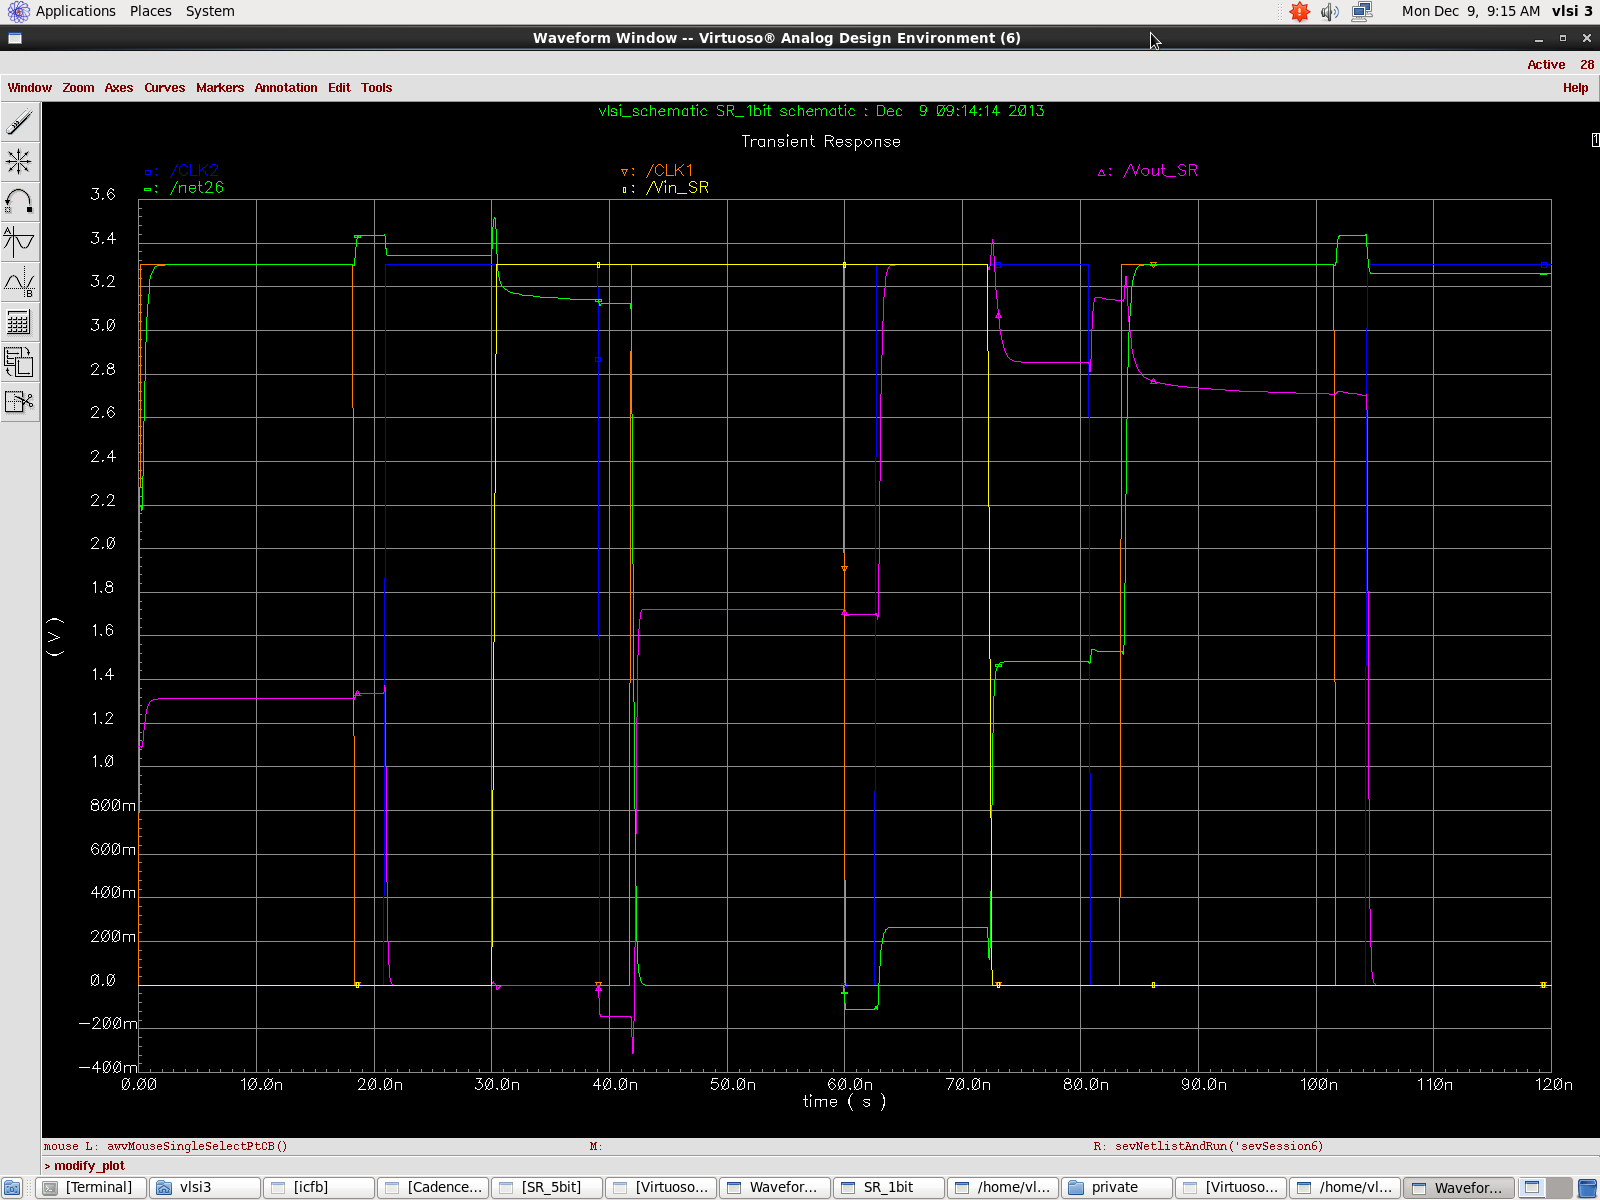
\includegraphics[width=0.7\textwidth]{wave_tussen1.png}
		\label{fig:wave_tussen1}
	}
	\subfigure[]{
		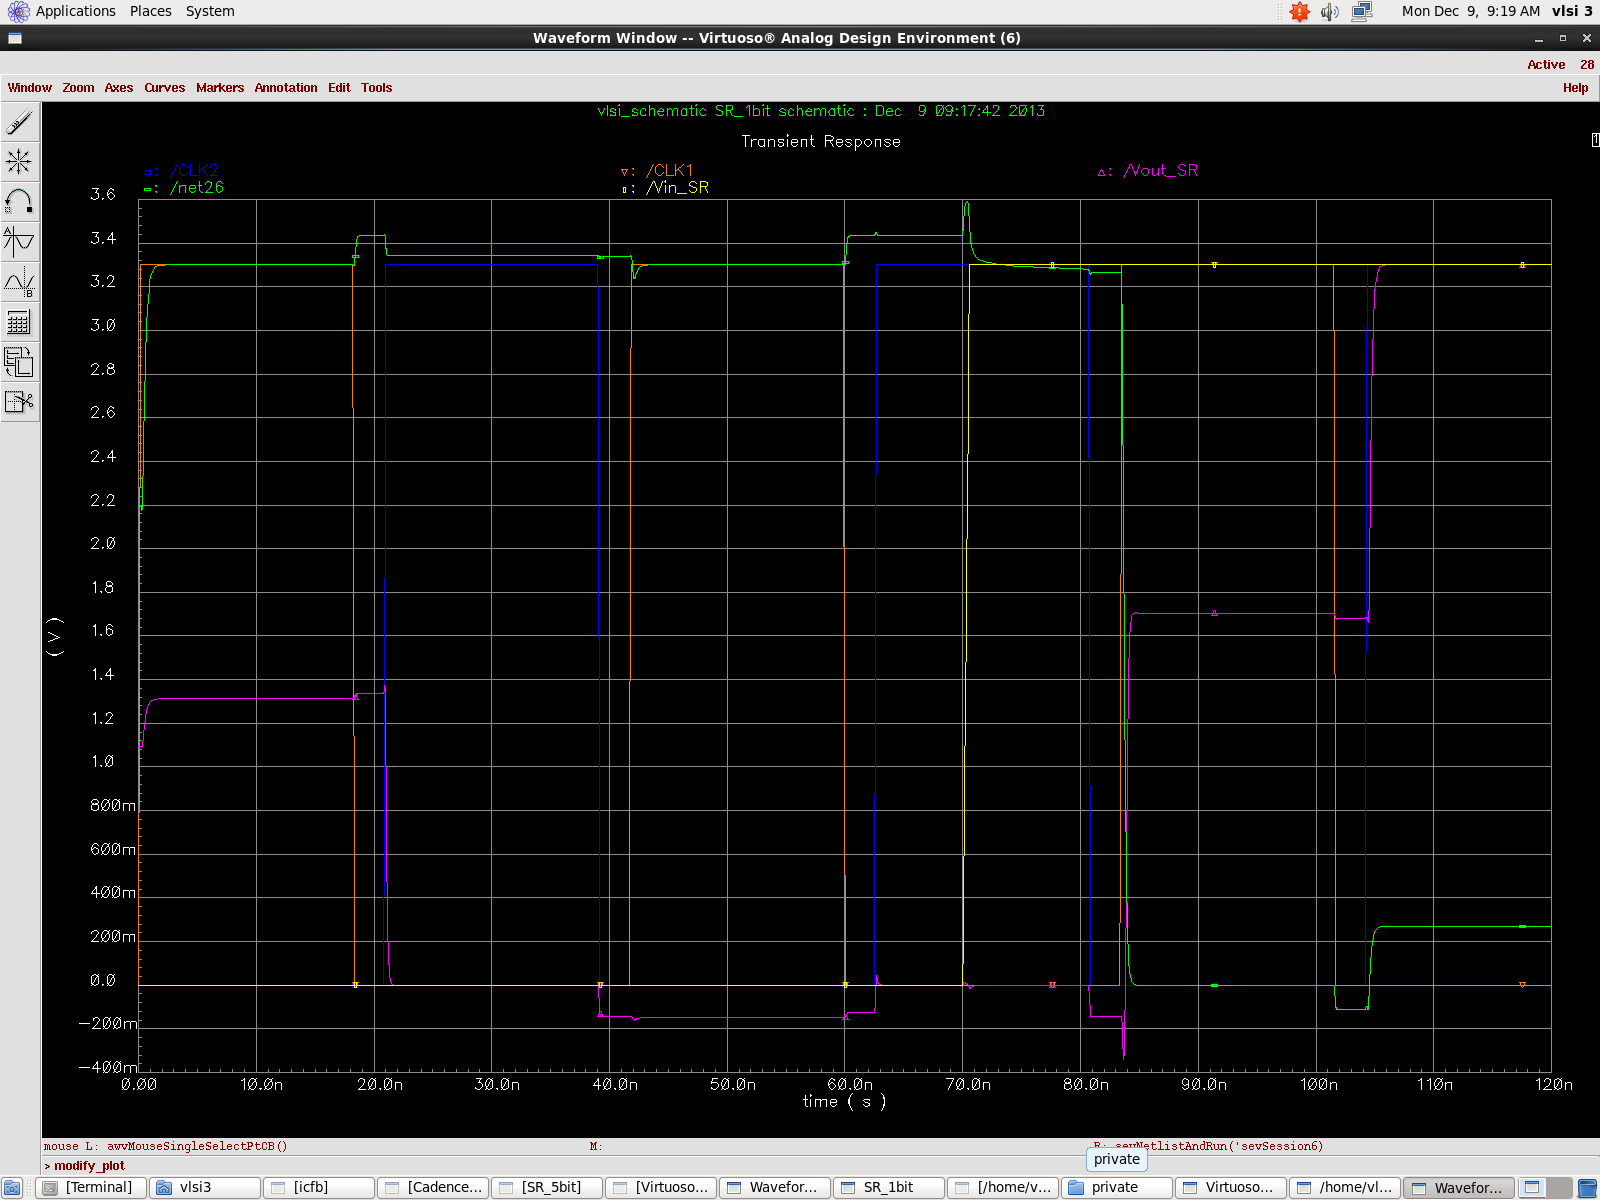
\includegraphics[width=0.7\textwidth]{wave_tussen2.png}
		\label{fig:wave_tussen2}
	}
	\caption{De werking van het 1-bit schuifregister voor twee verschillende ingangssignalen. net26 is de spanning $V_{tussen}$.}
	\label{fig:wave_tussen}
\end{figure}

De gate capaciteiten van $T_6$ en $T_7$ vormen de lastcapaciteiten van de eerste trap van het schuifregister. Om een symmetrische werking te verkrijgen, zorgen we ervoor dat deze lastcapaciteit niet afhangt van het type overgang. We kiezen dus

\begin{align*}
C_P &= C_N \\
\Leftrightarrow W_P L_P &= W_N L_N
\end{align*}

Bovendien willen we de factor $\frac{\sfrac{W_P}{L_P}}{\sfrac{W_N}{L_N}}$ gelijk houden aan $2,7$, zoals in de opgave. Wanneer we $W_P = L_N$ en $W_N = L_P$ gebruiken, is er nog een vrijheidsgraad die de tijdsconstante van het overgangsverschijnsel bepaalt. We kiezen als oplossing voor onze vergelijkingen:

\begin{align*}
W_N = L_P &= \SI{1}{\micro m} \\
W_P = L_N &= \SI{1,65}{\micro m}
\end{align*}

Door alle dimensies te vergroten met een factor $2$, is de invloed van een verandering op $V_{in}$ op $V_{tussen}$ kleiner. Het nadeel hiervan is dat de tijdsconstante van het overgangsverschijnsel groter wordt, maar dit is bij de gewenste frequentie geen probleem. De uiteindelijke parameters zijn:

\begin{align*}
W_N = L_P &= \SI{2}{\micro m} \\
W_P = L_N &= \SI{3,3}{\micro m}
\end{align*}

Figuur \ref{fig:wave_optimaal} toont de waveform van de 5-bit schakeling met deze waarden. Deze werkt nu zoals gewenst. Als maximale werkfrequentie vinden we ongeveer $\SI{125}{MHz}$. Om deze frequentie te bereiken, moet ervoor gezorgd worden dat de duty cycle van de kloksignalen voldoende dicht bij $50\%$ ligt.

\begin{figure}[htp]
	\centering
	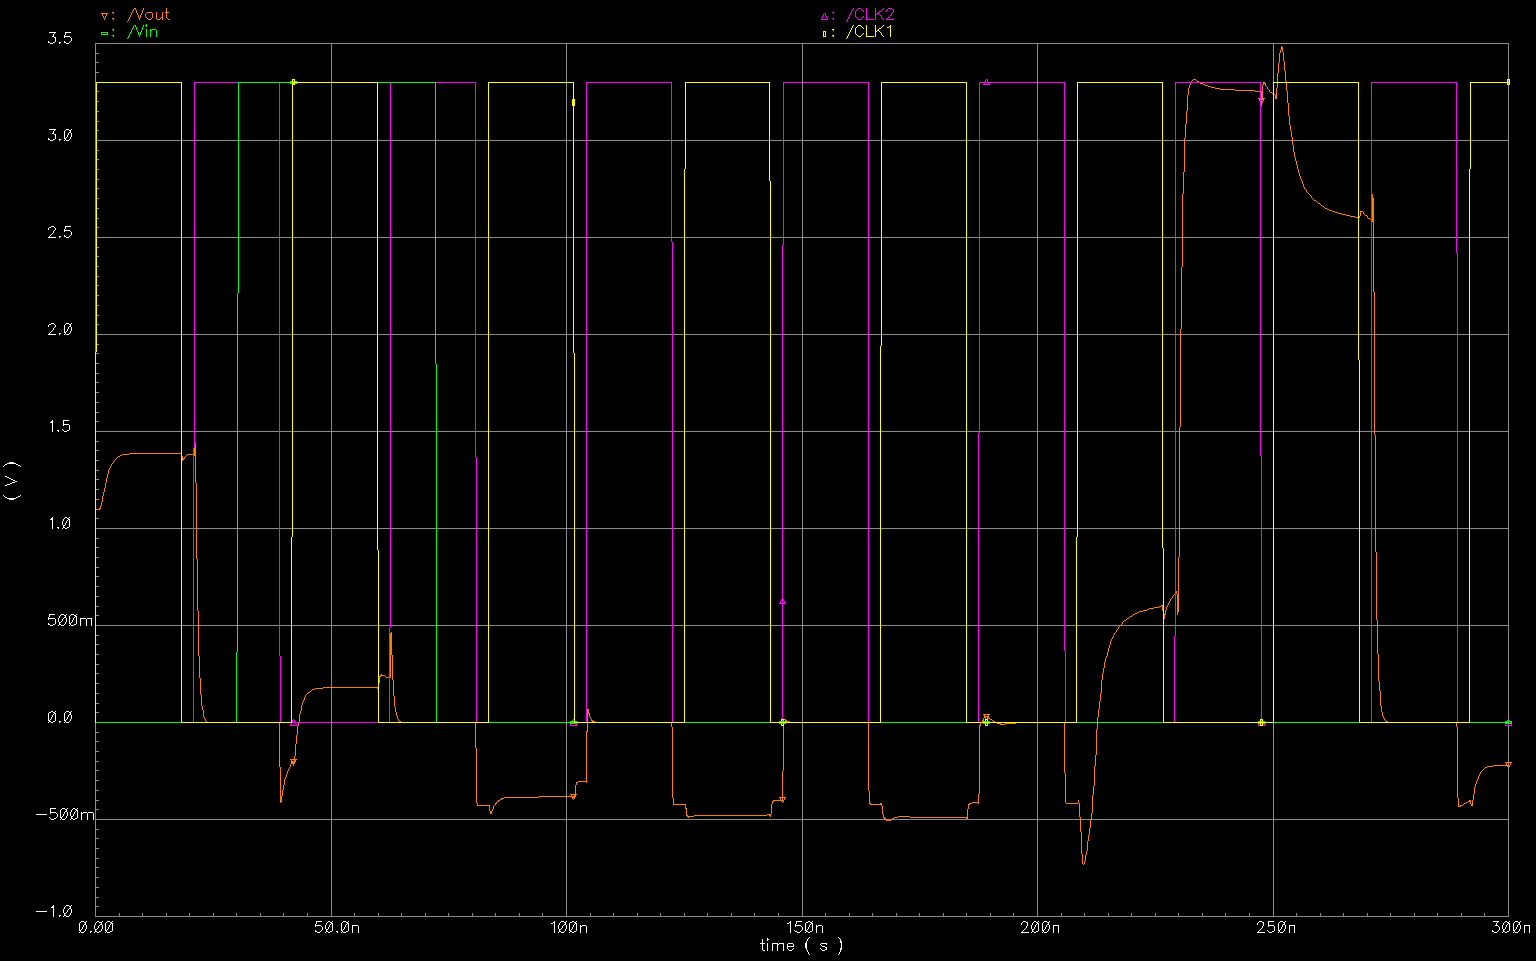
\includegraphics[width=0.7\textwidth]{wave_optimaal.png}
	\caption{De werking van het 5-bit register na correctie van de breedte en lengte van de transistors.}
	\label{fig:wave_optimaal}
\end{figure}

Als we de kloksignalen laten overlappen, huppelt het ingangssignaal te snel door de schakeling. Wanneer zowel $CLK_1$ als $CLK_2$ hoog is, kan het ingangssignaal van een schuifregister namelijk rechtstreeks doorstromen naar de uitgang. Figuur \ref{fig:wave_overlap} toont de waveform bij een duty cycle van $0,62$.

\begin{figure}[htp]
	\centering
	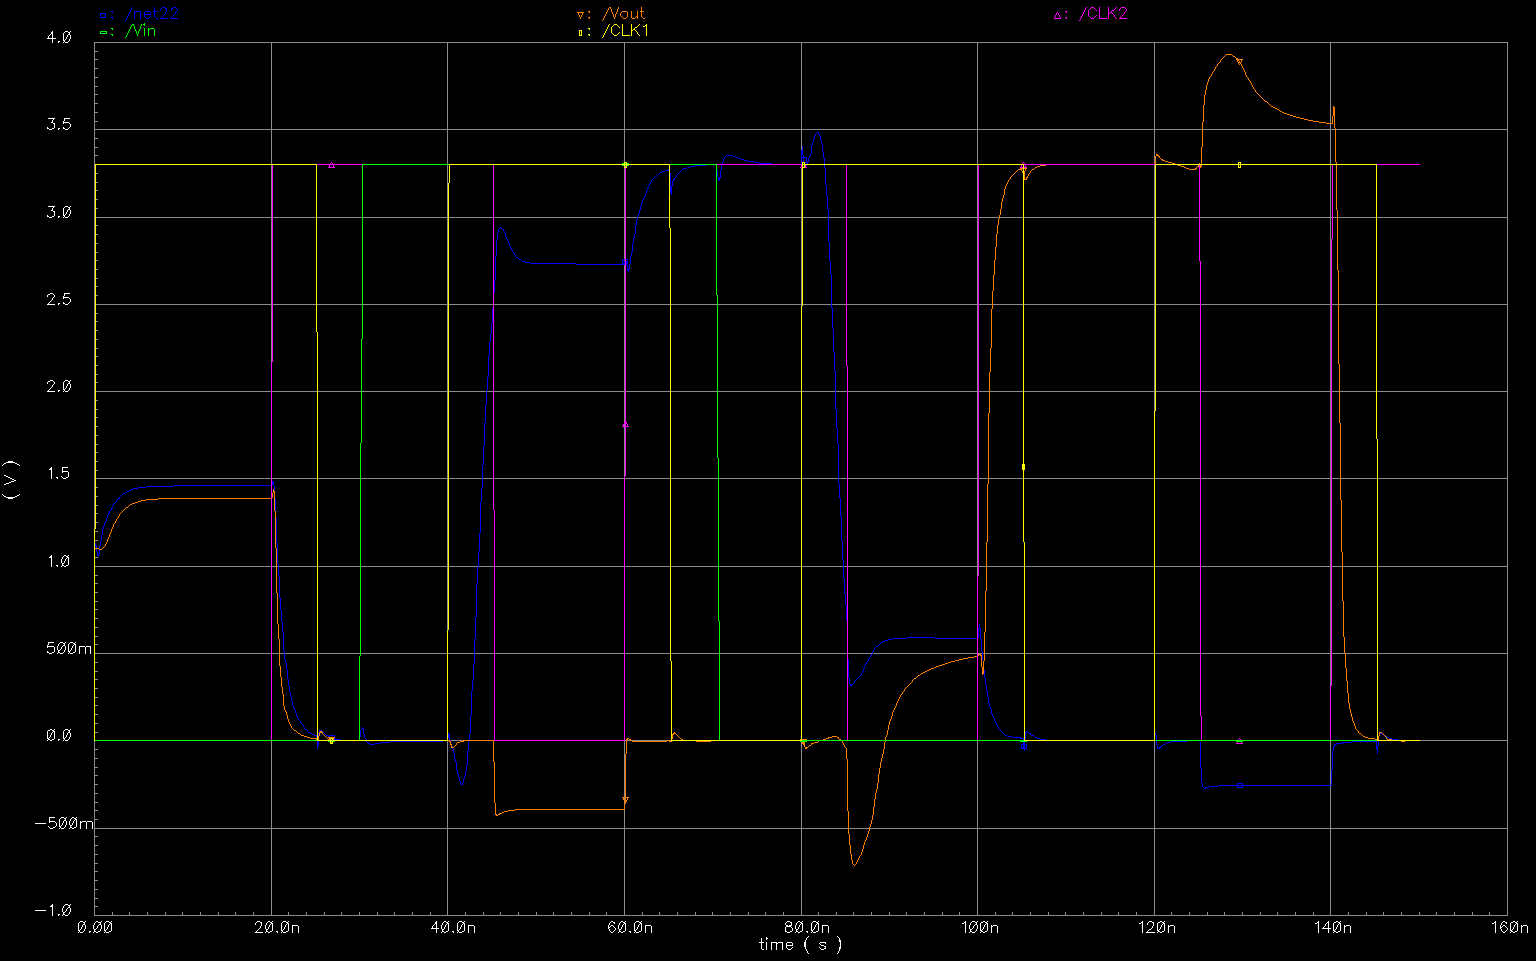
\includegraphics[width=0.7\textwidth]{wave_overlap.png}
	\caption{De werking van het 5-bit schuifregister bij overlappende kloksignalen. net22 is de uitgangsspanning van het eerste schuifregister.}
	\label{fig:wave_overlap}
\end{figure}



\section{Layout design}

Tijdens het tekenen van de layout van de invertor komen we één error tegen: de afstand tussen de poly en de naa mag niet groter zijn dan $2,2$. We verschuiven de gehele PMOS naar links om dit te verhelpen.

Bij het dimensioneren van de transistors hebben we geen rekening gehouden met de DRC-regels. Een kanaalbreedte van $\SI{2}{\micro m}$ is niet realiseerbaar. We herdimensioneren naar

\begin{align*}
W_N = L_P &= \SI{2,2}{\micro m} \\
W_P = L_N &= \SI{3,6}{\micro m}
\end{align*}

\end{document}